\input{~/github/config/preamble.sty}%available at github.com/danimalabres/config
\input{~/github/config/thms-eng.sty}%available at github.com/danimalabres/config


\usepackage[style=authortitle-terse,backend=bibtex]{biblatex}
\addbibresource{~/github/config/bibliography.bib}

\begin{document}

\begin{minipage}{\textwidth}
		Complex Manifolds in Dimension 1 \hfill Daniel González Casanova Azuela
		
		{Prof. Misha Verbitsky\hfill\href{https://github.com/danimalabares/riemann-surfaces}{github.com/danimalabares/riemann-surfaces}}
\end{minipage}\vspace{.2cm}\hrule

\vspace{10pt}
{\huge\bfseries Exam}

\tableofcontents

\addcontentsline{toc}{subsection}{Exercise 1.3}
\begin{manualexercise}{1.3}
	Let $M$ be an almost complex manifold, and $f:M\to \mathbb{R}$ a non-constant function which satisfies $d Jd(f)=0$. Prove that $M$ admits a non-zero holomorphic 1-form (this means closed form).
\end{manualexercise}

\begin{proof}[Solution]
	It is unclear what is the definition of a holomorphic form on an almost complex manifold. Here's some ideas:

	The form $\alpha:=df-\sqrt{-1}Jdf$ is complex linear since for any vector $v$
	\begin{align*}
		\alpha(Jv)&=\Big(df-\sqrt{-1}Jdf\Big)(Jv)\\
		&=df(Jv)-\sqrt{-1}df(J^2v)\\
		&=df(Jv)+\sqrt{-1}df(v)\\
		&=-\sqrt{-1}^2df(Jv)+\sqrt{-1}df(v)\\
		&=\sqrt{-1}\Big(df(v)-\sqrt{-1}d Jf(v)\Big)\\
		&=\sqrt{-1}\Big(df-\sqrt{-1}Jdf\Big)(v)\\
		&=\sqrt{-1}\alpha(v).
	\end{align*}

But then again it may be more suitable to find a form whose \textit{differential} is complex-linear. After consulting with Misha, he said to find a form that is closed… but $Jd(f)$ is already closed!
\end{proof}

\addcontentsline{toc}{subsection}{Exercise 1.7}
\begin{manualexercise}{1.7}
	Let $\eta$ be a closed 1-form on a 1-dimensional complex manifold $(M,I)$ such that $I(\eta)$ is also closed.

	\begin{enumerate}
		\item[a.] [Not part of the exam] Prove that $\eta=df$, where $f$ is a real part of a holomorphic function if $M$ is simply connected.

		\item[b.] Find an example of $(M,I,\eta)$ where $\eta$ is exact, but such $f$ does not exist.
	\end{enumerate}
\end{manualexercise}

\begin{proof}[Solution]\leavevmode 

	(See \href{https://math.stackexchange.com/questions/711950/show-omega-is-simply-connected-if-every-harmonic-function-has-a-conjugate}{StackExchange}.) The idea is to define the form as the exterior derivative of the real part of a logarithm. The logarithm cannot be defined globally so that function is not the real part of a holomorphic function.

	Summary: on any non-simply connected open subset $\Omega$ of $\mathbb{C}$ we can find a function, namely $u(z)=\log |z-w|$ with $w\notin \Omega$ such that there is a curve with nonezero winding number around it contained in $\Omega$. This function is harmonic but it is not the real part of a holomorphic function (which would be a complex logarithm).

	\begin{enumerate}[label=\textbf{Step \arabic*}]
		\item  Define $u(z)=\log|z-w|$ on a non-simply connected subset $\Omega\subset \mathbb{C}$ not containing $w$. Also let $\gamma$ be a curve with nonzero winding number with respect to $w$.
		
		\item Notice that $u$ is harmonic because it is \textit{locally} the real part of a holomorphic function, the logarithm.

		\item Suppose $v$ is such that $f:=u+iv$ is holomorphic. Recall that harmonic conjugates are unique up to adding a constant by Cauchy-Riemann equations. This means that the derivative of $f$ is the same as the detivative of the logarithm, ie., $f'(z)=\frac{1}{z-w}$.

	\item Remember the definition of the winding number:
	\[n(\gamma,w)=\frac{1}{2\pi i}\int_{\gamma}\frac{dz}{z-w}=\frac{1}{2\pi i}\int_{\gamma}f'\]
	so $n(\gamma,w)\neq0$ by the choices of $\gamma$ and $w$, but its also $0$ because it's the integral of a holomorphic function over a closed curve.
	\end{enumerate}



Now let's solve our exercise. Consider $\eta=du$ for the same $u$ as above. We already know that $u$ is not the real part of a holomorphic function but perhaps there is another function  $\tilde{u}$ such that $\eta= d\tilde{u}$ and $\tilde{u}$ is is the real part of a holomorphic function. Then $d(u-\tilde{u})=0$ {\color{6}so  $u-\tilde{u}$ is constant} so $\tilde{u}(z)=\log|z-w|+\lambda$. But the same argument shows that such a function cannot be the real part of a holomorphic function.

Let me be more clear about why $d(u-\tilde{u})=0\implies u-\tilde{u}$ is constant. $u(z)=\operatorname{log}|z-w|$ is a real function, and $\tilde{u}$ is also a real function by hypothesis. Now remember (see for example Huybrechts, \textit{Complex geometry} eq. 1.10 in p. 43) that the complex exterior differential is just the usual gradient; namely if $x+iy$ are coordinates of  $\mathbb{C}$, $df=\frac{\partial f}{\partial x}+\frac{\partial f}{\partial y}$ locally for a complex-valued function $f$ (just see Ahlfors p.27). Then
\[d(u-\tilde{u})= \frac{\partial }{\partial x}(u-\tilde{u})+ \frac{\partial }{\partial y}(u-\tilde{u})=\frac{\partial }{\partial x}(u-\tilde{u})\]
so that the gradient of $u-\tilde{u}$ is zero, Which means $u$ and  $\tilde{u}$ differ by a constant.
\end{proof}

\addcontentsline{toc}{subsection}{Exercise 2.7}
\begin{manualexercise}{2.7}
	Let $f_{i}$ be a collection of homolomorphic functions on a disk such that $\sum_{i=1}^{\infty} |f_{i}(z)|$ converges uniformly on $\Delta$. Prove that $\sum_{i=0}^{\infty}|f'(z)|$ converges uniformly on $\Delta$.
\end{manualexercise}

\begin{proof}[Solution]
	It looks like this is not always true. In my attempts of proving it I found a proof that $\sum_{i=0}^\infty f'(z)$ (without the bars) converges (uniformly) on $ \Delta$.


\addcontentsline{toc}{subsubsection}{A counter-example}
\vspace{1em}\textbf{A counter-example}

(See \href{https://math.stackexchange.com/questions/380446/prove-that-a-bounded-analytic-function-in-the-right-half-plane-which-vanishes-at}{StackExchange}). The counter example is
	\[f_n(z)=\frac{1}{n^2}\sqrt{1+z} \]
	First notice that the series of this function converges uniformly to $\pi^2/6\sqrt{1+z}$. This is just because $\sum 1/n^2$ converges to $\pi^2/6$ (this was proved first by Euler and apparently some people didn't believe him, see \href{https://math.stackexchange.com/questions/8337/different-ways-to-prove-sum-k-1-infty-frac1k2-frac-pi26-the-b}{here} for some proofs), and we can factor out of the series the term $\sqrt{1+z}$. To see convergence is uniform we simply note that $|\sqrt{1+z}|$ is bounded by 2 for all $z\in\Delta$.

	In turn, the series of derivatives is $\sum \frac{1}{2n^2}\frac{1}{\sqrt{1+z} }$ which converges to the derivative of series $\frac{\pi^2}{6}\frac{1}{\sqrt{1+z} }$ but not uniformly. To make sure suppose that for every $\varepsilon>0$ there is $N\in\mathbb{N}$ such that for every $n>N$ and  $z\in\Delta$ 
	\[\left| \frac{1}{2\sqrt{1+z} }\left( \frac{\pi^2}{6}-\sum_{i=1}^n\frac{1}{i^2} \right)  \right| <\varepsilon\]
	then
	\[\frac{1}{2\varepsilon}\left| \frac{\pi^2}{6}-\sum_{i=1}^n\frac{1}{i^2} \right|<|\sqrt{1+z} | \]
	but since we can take $z$ as close as $-1$ as we desire, the expression on the left is forced to be zero, which is not true.

	The reason is that the series converges to $\frac{\pi^2}{6}\sqrt{1+z} $, but the series of derivatives is unbounded, so "it cannot be uniformly convergent". But of course unboundedness alone does not imply that the sequence of derivatives cannot converge uniformly---for any unbounded function on a domain, just substracting a $1/n$-term will produce a uniformly convergent series of unbounded functions.
\vspace{1em}

\addcontentsline{toc}{subsubsection}{Proof of the statement without taking modulus}
\textbf{Proof of the statement without taking modulus}

Now I show how that if $\sum_{i=1}^{\infty} |f_{i}(z)|$ converges uniformly on $\Delta$, then$\sum_{i=0}^{\infty}|f'(z)|$ converges on $\Delta$.

	Recall from Alhfors \textit{Complex Analysis} (p. 176) Weierstrass theorem that if a sequence of holomorphic functions on a region $\Omega$ (a region is a nonempty connected open set) converges to a limit function $f$ in $\Omega$ and uniformly on every compact subset of $\Omega$, then  $f$ is analytic on $\Omega$. Moreover, $f'_{i}$ converges uniformly to $f'$ on every compact subset of $\Omega$.

	This is almost exactly what we need. Following I sketch the Ahlfor's proof slightly adapted to the exercise.


	Recall that an absolutely uniform convergent series is uniformly convergent, so that the sequence of partial sums $F_n=\sum_{i=1}^{n} f_i$ without the bars is uniformly convergent. Choose any point $z\in \Delta$ and a closed curve contained in $\Delta$ around $z$. Then Cauchy formula for the first derivative says $F'_{n}(z)=\frac{1}{2\pi i}\int_{\gamma}\frac{F_n(\zeta)}{(\zeta-z)^{2}}d\zeta$ for every $n \in \mathbb{N}$.
	%But we may also put the bars to get $|F'_{n}(z)|=\left|\frac{1}{2\pi i}\int_{\gamma}\frac{F_n(\zeta)}{(\zeta-z)^{2}}d\zeta\right|$ for every $n \in \mathbb{N}$. 
	Now take limit and put it inside the integral using uniform convergnce of $F_n$ to get that
	\begin{align*}
	\sum_{i=1}^{\infty} f_i' &=\frac{1}{2\pi i}\int_{\gamma}\frac{\sum_{i=1}^{\infty} f_i(\zeta)}{(z-\zeta)^{2}}d\zeta\\
	%&=\left| \frac{1}{2\pi i}\int_{\gamma} \right|
\end{align*}
which says that $\sum_{i=1}^{\infty} f'$ converges to the derivative of $\sum_{i=1}^{\infty} f$. Then Ahlfors says a simple estimate shows convergence is uniform but I'm not sure how exactly.
\end{proof}

\addcontentsline{toc}{subsection}{Exercise 2.8}
\begin{manualexercise}{2.8}
	Construct a non-zero bounded homolomorphic function on $\{z\in \mathbb{C}:\operatorname{Re}(z)>0\} $ such that $f(n)=0$ for all $n \in \mathbb{Z}^{>0}$.
\end{manualexercise}

\begin{proof}[Solution]\leavevmode 
	(See \href{https://math.stackexchange.com/questions/380446/prove-that-a-bounded-analytic-function-in-the-right-half-plane-which-vanishes-at}{StackExchange}) Such a function doesn't exist. We will show it must be constant.
\begin{enumerate}[label=\textbf{Step \arabic*}]
		\item Pass to a function whose domain is the unit disk by composing $f$ with a M\"obius transformation that maps the disk to the right-hand plane, namely $z\mapsto \frac{1}{1+z}-\frac{1}{2}$. So define $g(z)=f\left( \frac{1}{1+z}-\frac{1}{2} \right) $.

	$g(z)=0$ when $\frac{1}{1+z}-\frac{1}{2}$ is an integer $n$ so define $z_{n}=-1+\frac{1}{n+\frac{1}{2}}$.

		\item $\prod_{n} |z_{n}| $ diverges to zero. That means that it converges to zero but the infinite sum (series) the logarithms diverges.
\clearpage
\begin{thing4}{Exercise 8}[\cite{zo1}, 3.2.5, p. 148]\leavevmode
An inifinite product $\prod_{k=1}^\infty e_k$ is said to converge if the sequence $\Pi_n=\prod_{k=1}^n e_k$ has a finite \textbf{nonzero} limit $\Pi$. We then set $\Pi=\prod_{k=1}^\infty e_k$. Show that
\begin{enumerate}[label=(\alph*)]
	\item[(b)]  if $\forall n \in N (e_n>0)$, then the infinite product converges $\prod_{n=1}^\infty$ converges if and only if the series  $\sum_{n=1}^\infty \operatorname{log}e_n$ converges.
\end{enumerate}
\end{thing4}

\begin{remark}\leavevmode
The proof is straightforward using elementary properties of the logarithm ($\operatorname{log}(ab)=\operatorname{log}a+\operatorname{log}b$) and the exponential ($\operatorname{exp}(a+b)=\operatorname{exp}a+\operatorname{exp}b$), as well as their continuity. The caveat is that if the product converges to zero, taking logarithms of the partial products gives a series diverging to $-\infty$ (we say that the product \textit{\textbf{diverges to zero}}). The following exercise is an example of this.
\end{remark}

\begin{claim}\leavevmode
\begin{align*}
			\prod_{n\geq 0}\left|  -1+\frac{1}{n+\frac{1}{2}}\right|=0.
				\end{align*}
\end{claim}			
\begin{proof}\leavevmode
By taking exponent of the partial sums of the following series, we see it's enough to show that
\begin{equation}\label{eq:log}\sum_{n \geq 0}\operatorname{log}\left|  -1+\frac{1}{n+\frac{1}{2}}\right|=-\infty.
\end{equation}
To show this first notice that $\left|  -1+\frac{1}{n+1/2}\right|$ is just  $1-\frac{1}{n+1/2}$. We can also quickly notice that $\operatorname{log}\left(1-\frac{1}{n+1/2}\right)$ is a sequence of negative numbers convering to 0.

(It was not immediate to me why the this series should diverge or converge. The following argument was provided by ChatGPT.)

We can prove the series diverges if we find a divergent series that bounds it from above. Such series is $\sum\frac{-1}{n+1/2}$. Indeed, it turns out that for every number $0\leq x<1$,
\[\operatorname{log}(1-x) \leq -x.\]
To see why, define the function $f(x)=\operatorname{log}(1-x)+x$ and differentiate to find
\[\frac{d}{dx}\operatorname{log}(1-x)+x=-\frac{1}{1-x}+1=\frac{1}{1-x}+\frac{1-x}{1-x}=\frac{-x}{1-x}\leq 0,\]
and since also $f(0)=0$, we have that
\[\operatorname{log}(1-x)+x\leq 0,\qquad 0\leq x<1.\]
Finally just recall that $\sum_{n\geq 0}\frac{1}{n}$ diverges (and behaves like $\sum \frac{1}{n+1/2}$ for lage $n$). This confirms \cref{eq:log}.




\end{proof}
\clearpage
		\item Consider the inverse of a finite Blaschke product that vanishes on the $z_{n}$ (this is why we put everything inside the unit disk). It is $\tilde{B}_{k}(z)=\prod_{n=1}^{k} \frac{1-z\cdot z_{n}}{z-z_{n}}  $. Also consider the product $g\cdot \tilde{B}_{k}$, which is analyitic because $g$ vanishes at the poles of $\tilde{B}_{k}$.
\begin{figure}[H]
	\centering
	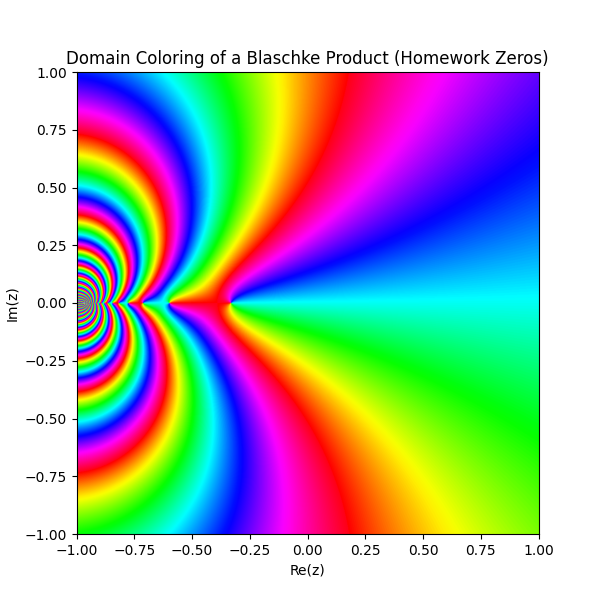
\includegraphics[width=0.3\textwidth]{Figure_1.png}
	\caption{Domain coloring plot for $\tilde{B}$}
\end{figure}

		\item Recall that the modulus of such a function takes its maximum at the boundary of its domain. Then show that $|\tilde{B}_{k}(z)|$ is bounded by 1 (I'm not sure how). We already know that $g$ is bounded by some number $M$ because $f$ is bounded by hypothesis. We have $|g(z)| \leq \frac{M}{|\tilde{B}_{k}(z)|}$ for all $|z|<1$ and all $k$.

		\item Put $z=0$, you get $|g(z)| \leq M\cdot \prod_{n\leq k} |z_{n}| $ and take limit as $k\to \infty$. The product diverges to zero so $g(0)=0$.

		\item That means $\frac{g(z)}{z}$ is analytic so do everything again with $\frac{g(z)}{z}$ instead of $g(z)$. And again for $\frac{g(z)}{z^{2}}$. And so on. $g$ has a zero of infinite order, which is not possible and thus it is constant zero.
	\end{enumerate}
\end{proof}

\addcontentsline{toc}{subsection}{Exercise 3.3}
\begin{manualexercise}{3.3}
	Let $V$ be an $n$-dimensional Hermitian complex space of signature $(1,n-1)$. Prove that the space $B\subset \mathbb{P}_{\mathbb{C}}V$ of all positive complex lines in $V$ biholomorphic to a ball in $\mathbb{C}^{n-1}$.
\end{manualexercise}

\begin{proof}[Solution]
	(See \href{https://en.wikipedia.org/wiki/Complex_hyperbolic_space#Projective_model}{Wiki}.) A positive line is a 1-dimensional subspace $\ell$ such that $q(x,x)>0$ for some (and hence all) $x\in \ell$. For a line to be positive there must be a representative with non-zero first coordinate, which we may choose (uniquely) to be 1. Then
	\[q(x,x) >0\quad \iff\quad 1>\sum_{i=2}^{n} |x_i|^2.\]
We have constructed a biholomorphism
\begin{align*}
	B &\longrightarrow \{ |x|<1\} \subset \mathbb{C}^{n-1} \\
	[1:x_2:\ldots:x_n] &\longmapsto (x_2,\ldots,x_n)
\end{align*}

\end{proof}

\begin{manualdef}{3.1}
	\textit{\textbf{Horocycle}} on a Poincar\'e plane is an orbit of a parabolic subgroup
	\[P_{t}=\begin{pmatrix}1&t\\0&1\end{pmatrix}\in \operatorname{PSL}(2,\mathbb{R})=\operatorname{SO}^{+}(1,2). \]
\end{manualdef}

\addcontentsline{toc}{subsection}{Exercise 3.7}
\begin{manualexercise}{3.7}
	Prove that the group of isometries $\operatorname{Iso}(\mathbb{H}^{2})=\operatorname{SO}^{+}(1,2)$ acts transitively on the set of horocycles.
\end{manualexercise}

\begin{proof}[Solution]
	Let's fix two parabolic subgroups. I say that there is an isometry in $\operatorname{Iso}(\mathbb{H}^2)$ that maps one to the other via conjugation. This gives a transitive action on horocycles: two horocycles, each determined by a point and a parabolic subgroup, are paired via a single element of $\operatorname{Iso}(\mathbb{H}^2)$ (the pairing is via conjugation on subgroups and usual mapping on points).
\end{proof}

\addcontentsline{toc}{subsection}{Exercise 4.2}
\begin{manualexercise}{4.2}
	Let $M$ be a compact, Kobayashi-hyperbolic complex manifold. Prove that $M$ does not admit non-zero holomorphic vector fields.
\end{manualexercise}

\begin{proof}[Solution]\leavevmode

Integrating a non-zero vector field on $M$ gives a complex 1-parameter subgroup acting on $M$. Let's show that $\mathbb{C}$ cannot act nontrivially on $M$. Suppose that $f:\mathbb{C}\times M\to M $ is an holomorphic action of $\mathbb{C}$ on $M$. Then for each $p\in M$, the map $a\in\mathbb{C}\mapsto f(a,p)\in M$ is holomorphic, so it is distance decreasing with respect to Kobayashi distances in $\mathbb{C}$ and $M$ (i.e. it is 1-Lipschitz). But Kobayashi distance in $\mathbb{C}$ is trivial, making the action trivial.
\end{proof}

\addcontentsline{toc}{subsection}{Exercise 4.6}
\begin{manualexercise}{4.6}
	Let $a,b,c\in \operatorname{Abs}$ be three distinct points on the absolute, and $A\in \operatorname{SO}^{+}(1,2)$ an isometry of Poincar\'e plane which fixes $a,b,c$. Prove that $A=\operatorname{Id}$.
\end{manualexercise}

\begin{proof}[Solution]
	We have seen in our lectures that $\operatorname{SO}^{+}(1,2)$ is isomorphic to the group of transformations $z\mapsto \frac{az+b}{cz+d}$ with $a,b,c,d\in \mathbb{R}$ and $ad-bc>0$. Such transformations act on the upper-half plane as hyperbolic isometries.  A fixed point of any such transformation is solution of a quadratic equation, which has potentially only two distinct solutions. Thus, if a transformation fixes three distinct points, it must be the identity.
\end{proof}

\addcontentsline{toc}{subsection}{Exercise 5.2}
\begin{manualexercise}{5.2}
	Let $M$ be a Riemann surface with infinite fundamental group. Prove that any continuous map $S^{2}\to M$ is homotopic to a trivial map (map to a point).
\end{manualexercise}

\begin{proof}[Solution]
%	Let's see what's up with the induced map $\pi_{1}(S^{2})\to \pi_{1}(M)$. Well it is trivial because $S^{2}$ is simply-connected.

	{\color{4}\bfseries Solution using Uniformization theorem.}\hspace{.5em}All higher homotopy groups of Riemann surfaces of nonzero genus are trivial by covering space argument (covering space is contractible by Uniformization theorem). For $S^{2}$ itself, the statement does not hold since it would imply that $-\operatorname{Id}$ is homotopic to $\operatorname{Id}$, which is not true (but of course, the fundamental group of $S^2$ is not infinite).

	{\color{4}\bfseries Solution using Witehead theorem.}\hspace{.5em}Universal cover $U$ is contractible by Witehead theorem. Indeed, a point and $U$ are weakly homotopically equivialent (=all homotopy groups are the same). $\pi_{1}(U) =0$ by universal cover being simply connected. To see that all other homotopy groups vanish use Hurewicz to notice that if one of them was nonzero it would be isomorphic to the homology group in the corresponding degree. But  $U$ is acyclic (=all homology groups vanish). Above degree 2 it is clear by dimension, and for degree 2 use Poincaré duality with compact support to see that $H_2(U)=H^{0}_c(U)$. However, the definition of $H^{2}(M)$ is the set of cohomology classes of smooth real-valued locally constant (since they satisfy $df=0$) functions with compact support. Now this group is trivial beacuse $U$ cannot be compact, which in turn is because the fundamental group of the Riemann surface is infinite and the universal cover is a discrete cover.

{\color{4}\bfseries A more elementary proof?}\hspace{.5em}Let $f:S^2\longrightarrow M$ be any continuous map. The induced map on fundamental groups is $f^* :\pi_{1}(S^2) \longrightarrow \pi_{1}(M)$ but $\pi_{1}(S^2)$ is trivial, there exists a lift $\tilde{f}$ to any covering space. Also we have an action of $\pi_{1}(M)$ on the universal cover, so that we have infinitely many copies of $\tilde{f}(S^2)$ in the universal cover.

\end{proof}

\addcontentsline{toc}{subsection}{Exercise 5.8}
\begin{manualexercise}{5.8}
	Let $TS^{2}\oplus C^{\infty} S^{2}$ be a direct sum of a tangent bundle $TS^{2}$ and a 1-dimensional bundle. Is the bundle $TS^{2}\oplus C^{\infty} S^{2}$ trivial?
\end{manualexercise}

\begin{proof}[Solution]
	[From Hatcher VBK p. 10.] The direct sum of $TS^{2}$ and its normal bundle $NS^{2}$ is trivial since the map $(x,v,tx)\mapsto (x,v+t x)$, with $v$ tangent at $x\in S^{2}$ and $t\in \mathbb{R}$, is an isomorphism $TS^{2}\oplus NS^{2}\cong S^{2}\times \mathbb{R}^{3}$. The idea here is that while any global section will vanish at one point $x\in S^{2}$, so $v_{x}=0$, the point $x$ will never be zero.

	Recall that a vector bundle isomorphism consists of an homeomorphism of the total spaces that restricts to a linear isomorphism between corresponding fibers. It is clear that the map above is an homeomorphism, and fixing $x \in S^{2}$ we also find a trivial isomorphism between the fibers---there isn't much to say here.

	For a line bundle $C^{\infty} S^{2}$ that is always linearly independent with respect to $TS^{2}$ (which is the case since we have a direct sum), the map $(x,v,y)\mapsto (x,v+y)$ yields an isomorphism $TS^{2}\oplus C^{\infty} \cong S^{2}\times \mathbb{R}^{2}$ or $S^{2}\times \mathbb{R}^{3}$ depending on the rank of $TS^{2}$.
\end{proof}

\end{document}
